\documentclass[aspectratio=169,11pt]{beamer}

\usetheme{Madrid}
\usecolortheme{default}
\usefonttheme{professionalfonts}
\setbeamertemplate{navigation symbols}{}
\setbeamertemplate{footline}[frame number]

\usepackage{amsmath, amssymb, booktabs, graphicx}
\graphicspath{{../../assets/figures/}{assets/figures/}}

\title{Households, Family, Fertility, and Time Allocation}
\subtitle{Labor I --- Week 6}
\author{Teaching deck draft}
\date{}

\begin{document}

\begin{frame}
  \titlepage
\end{frame}

\begin{frame}{Central question and motivation}
\begin{itemize}
    \item Week 6 asks how households transform wage opportunities into realized hours, earnings, and career paths.
    \item Children and care needs reallocate time, not only tastes.
    \item Family policy matters for labor markets because it changes household production, bargaining, and dynamic career interruption.
\end{itemize}
\end{frame}

\begin{frame}{Week 5 to Week 6 bridge}
\begin{itemize}
    \item Week 5 treated wages as market opportunities tied to skill and sorting.
    \item Week 6 asks why similar wage opportunities can produce different labor outcomes once partners, children, and care constraints enter.
    \item The relevant decision-making unit is often the household even when the data are person-level.
\end{itemize}
\end{frame}

\begin{frame}{Household time-allocation problem}
\[
T_i = h_i + n_i + \ell_i
\]

\begin{itemize}
    \item Market work \(h_i\), home production or care \(n_i\), and leisure \(\ell_i\) compete for the same time endowment.
    \item A birth shock changes the shadow value of \(n_i\), not only the wage response along a standard labor-supply curve.
    \item Household-service substitutes and childcare access therefore matter for labor supply even when wages do not move.
\end{itemize}
\end{frame}

\begin{frame}{Household time allocation before and after childbirth}
\begin{center}
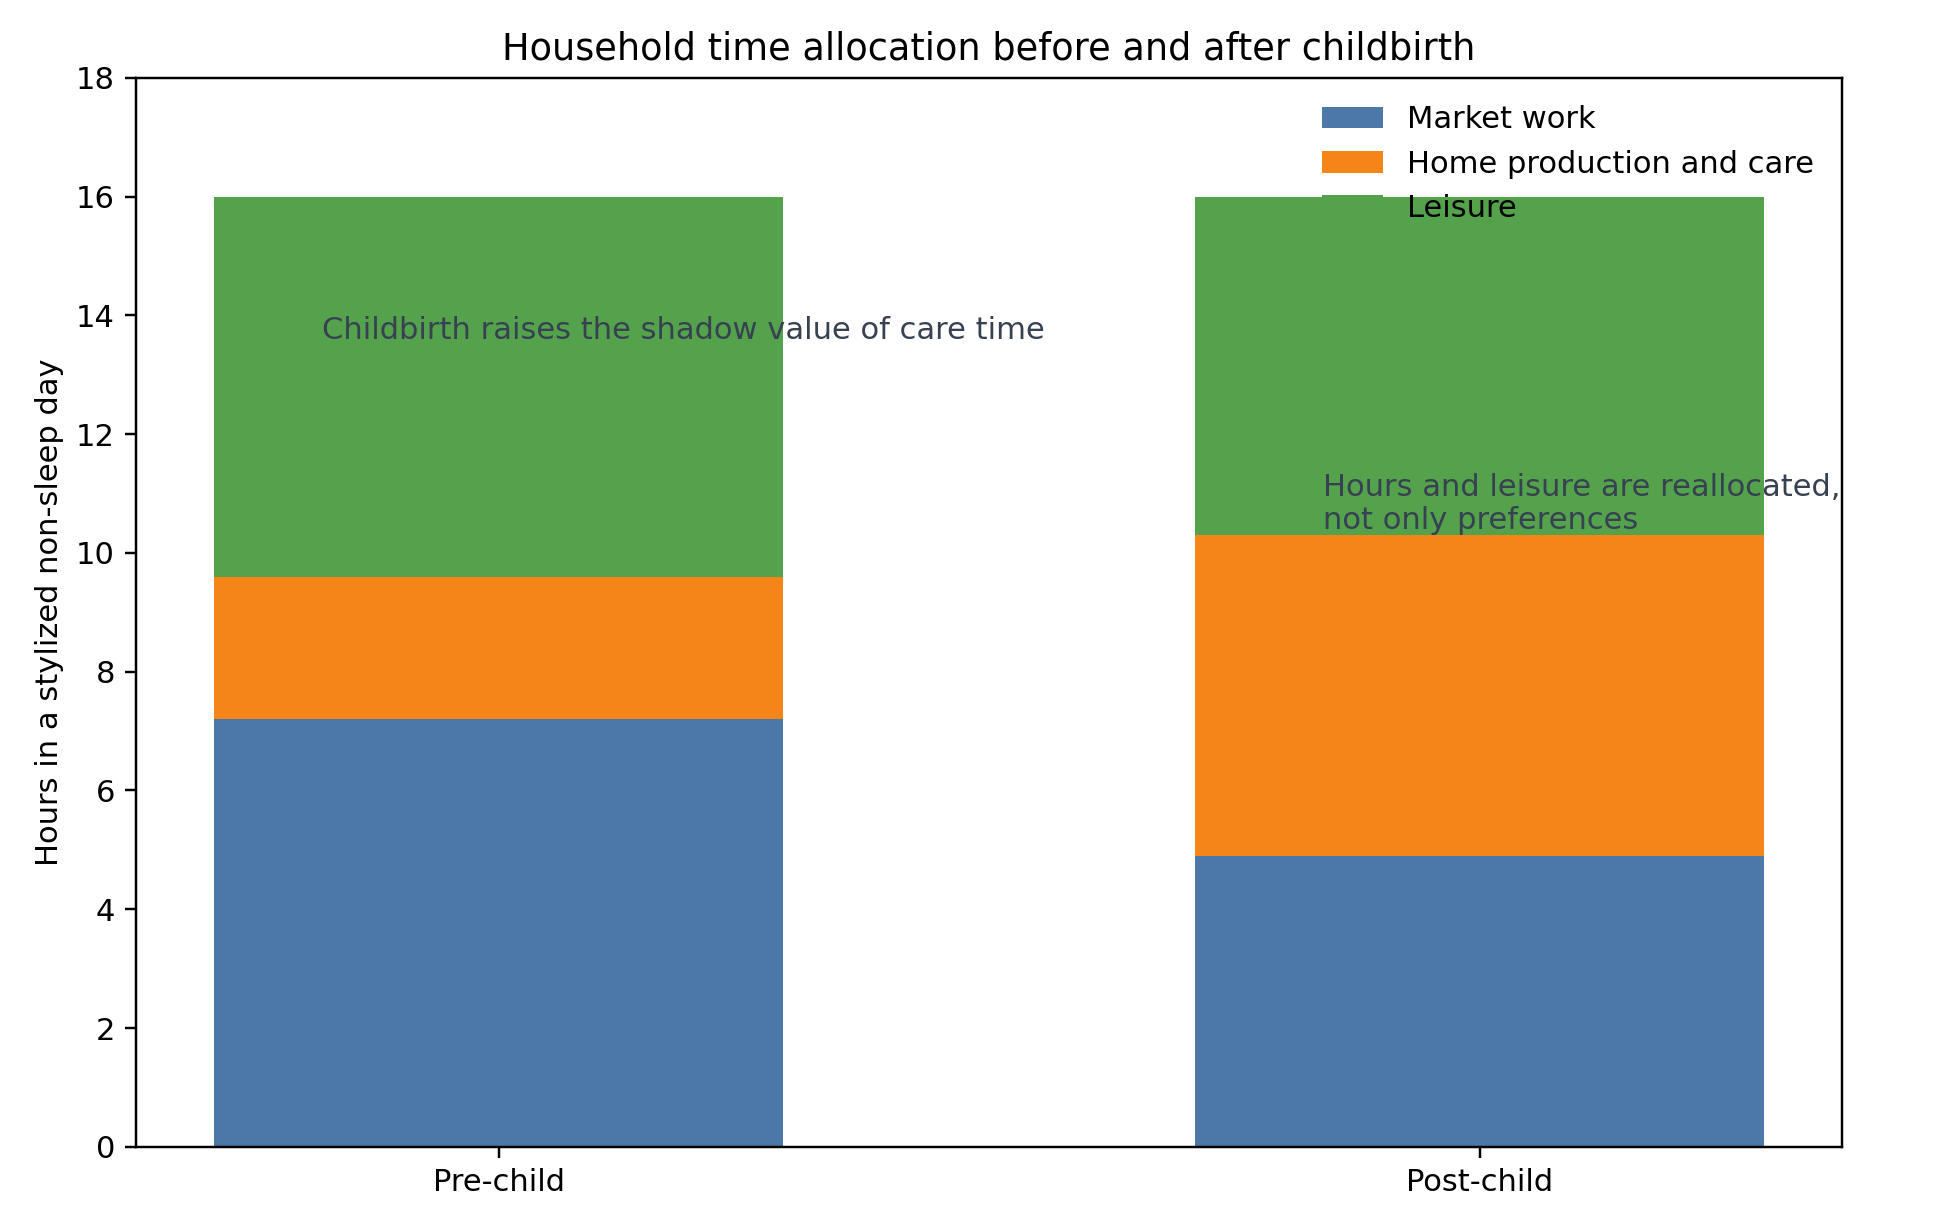
\includegraphics[height=0.74\textheight,keepaspectratio]{06-household-time-allocation-schematic.png}
\end{center}
\end{frame}

\begin{frame}{Household production and market substitutes}
\[
\max U(c_f, c_m, \ell_f, \ell_m, q)
\quad
\text{s.t.}
\quad
c_f + c_m + p_x x = w_f h_f + w_m h_m + y,
\quad
q = F(n_f, n_m, x)
\]

\begin{itemize}
    \item The household good \(q\) can be produced with parental time or market inputs \(x\).
    \item Lower \(p_x\) relaxes the home-production constraint and can raise market hours.
    \item Gelbach and Cort\'es--Tessada are clean empirical versions of this comparative static.
\end{itemize}
\end{frame}

\begin{frame}{Childcare and outsourcing as labor-supply shifters}
\begin{center}
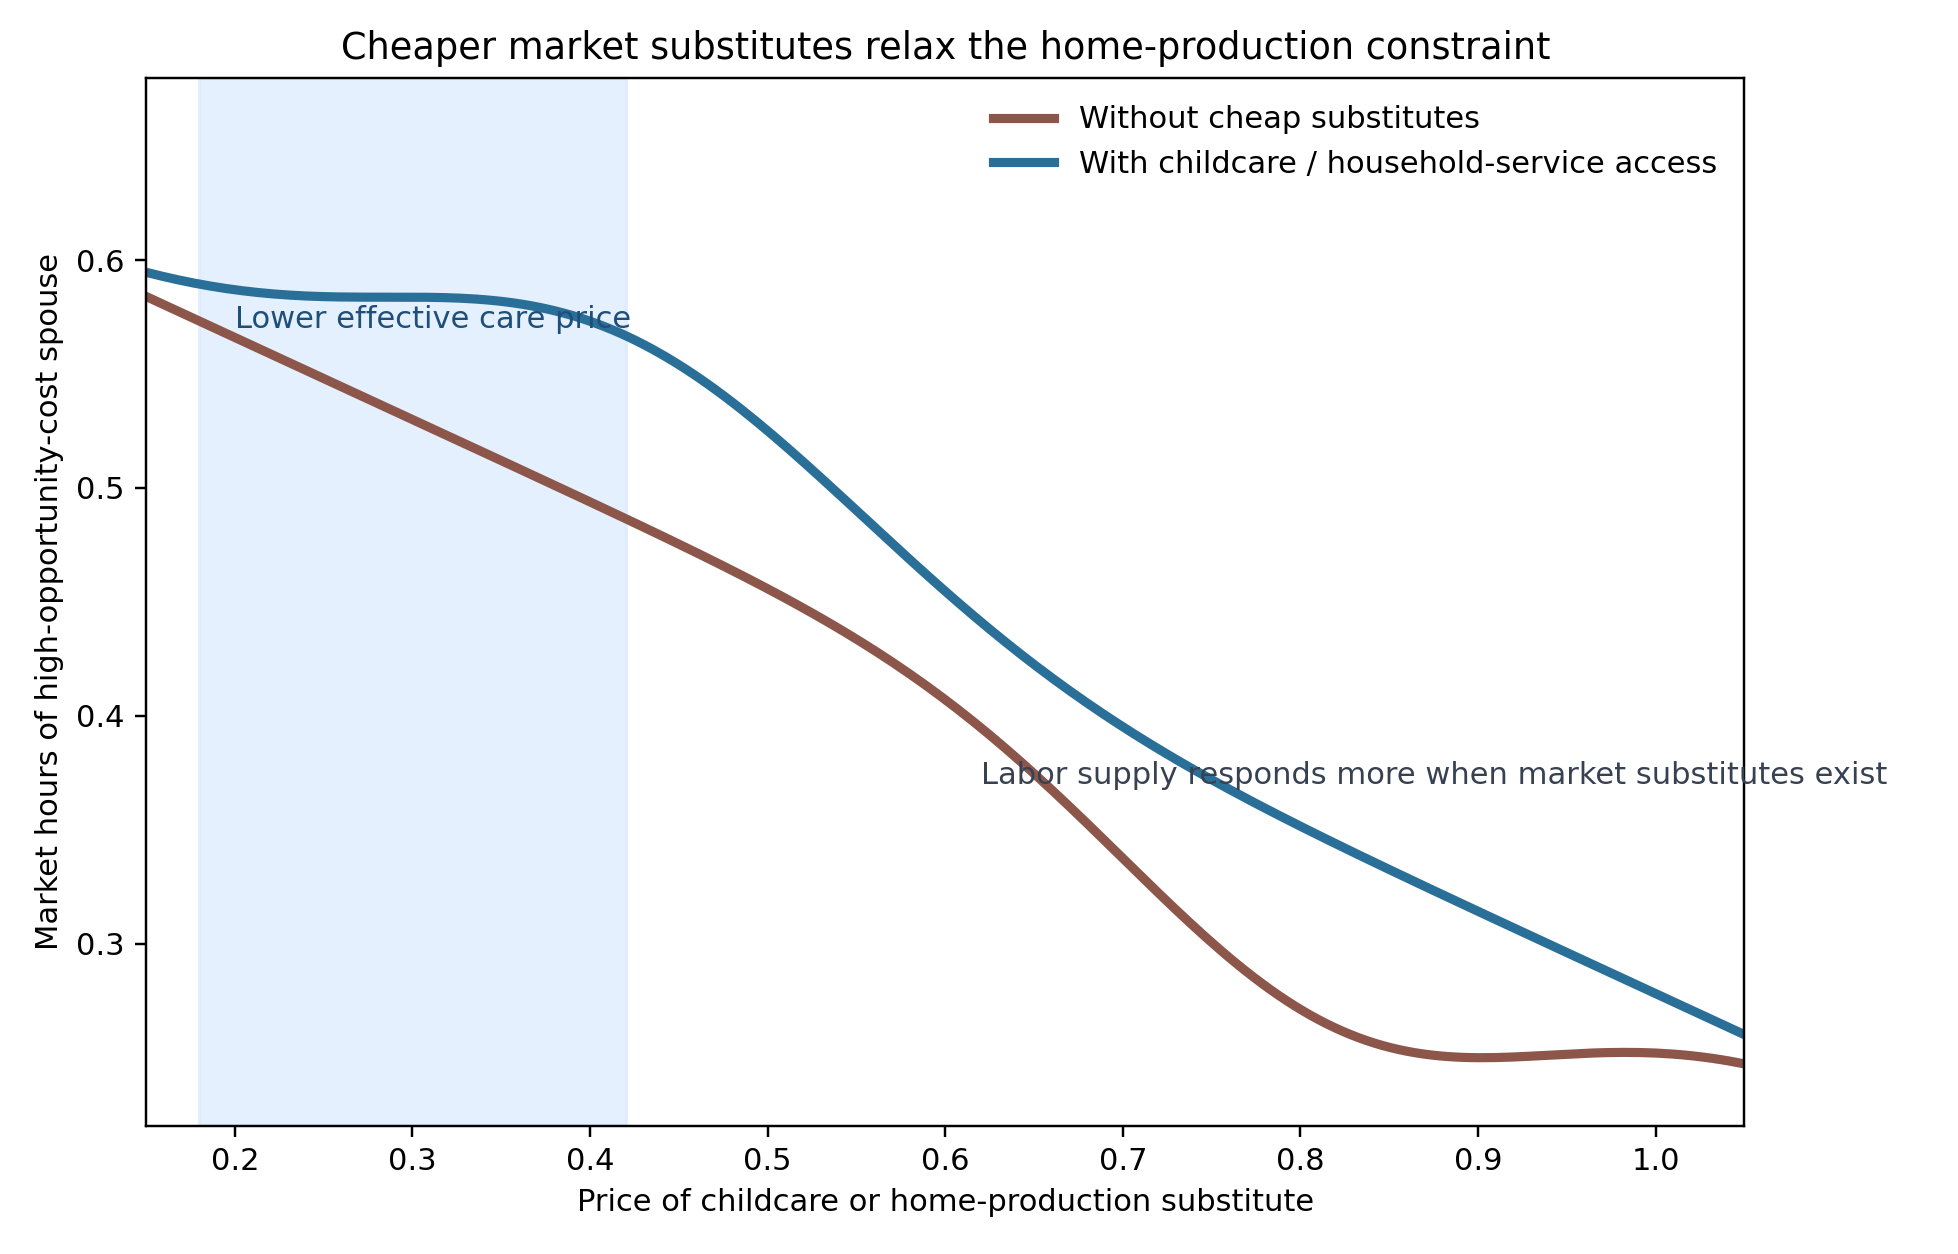
\includegraphics[height=0.74\textheight,keepaspectratio]{06-childcare-substitution-schematic.png}
\end{center}
\end{frame}

\begin{frame}{Unitary versus collective household models}
\[
\max \lambda U_f(\cdot) + (1-\lambda) U_m(\cdot)
\]

\begin{itemize}
    \item Unitary models pool resources and act as a clean benchmark.
    \item Collective models keep efficiency but allow the sharing rule \(\lambda\) to respond to distribution factors.
    \item Policy incidence can therefore depend on who receives transfers, not only on total family income.
\end{itemize}
\end{frame}

\begin{frame}{Household-model map}
\scriptsize
\begin{tabular}{p{0.18\linewidth} p{0.20\linewidth} p{0.20\linewidth} p{0.18\linewidth} p{0.17\linewidth}}
\toprule
Bucket & Choice object & Variation or test & Good for & Caveat \\
\midrule
Unitary & Pooled utility & Income pooling restrictions & Benchmark family labor supply & Too restrictive when recipient matters \\
Collective & Sharing rule \(\lambda\) & Distribution factors & Incidence and bargaining & Requires richer structure \\
Household production & Work, care, leisure, substitutes & Care prices and time prices & Care constraints and outsourcing & Home production hard to measure \\
Fertility IV & Extra child margin & IVF success or similar variation & Causal fertility effects & Local margin only \\
Child event study & Dynamic post-birth path & Event time around first birth & Persistent child penalties & Not an automatic policy counterfactual \\
Policy designs & Childcare, leave, transfers & Reform timing or eligibility & Policy incidence on labor outcomes & Multiple margins often move together \\
\bottomrule
\end{tabular}
\end{frame}

\begin{frame}{Fertility and childbirth as labor-market shocks}
\begin{itemize}
    \item Childbirth changes participation, hours, occupation choice, firm attachment, and later wage growth.
    \item Lundborg, Plug, and Rasmussen isolate a fertility margin through IVF treatment success.
    \item The resulting estimand is a local causal effect of an additional child, not a complete dynamic child-penalty path.
\end{itemize}
\end{frame}

\begin{frame}{Child-penalty event-study object}
\[
Y_{it} = \sum_{k \neq -1} \beta_k \mathbf{1}\{t - b_i = k\} + \alpha_i + \gamma_t + \varepsilon_{it}
\]

\begin{itemize}
    \item The \(\beta_k\) coefficients trace the full path relative to the pre-birth period.
    \item Kleven, Landais, and Sogaard show that the divergence is persistent and tied to career dynamics, not only contemporaneous hours.
    \item This is why Week 6 is a bridge into inequality rather than only a family-policy week.
\end{itemize}
\end{frame}

\begin{frame}{Stylized child-penalty event study}
\begin{center}
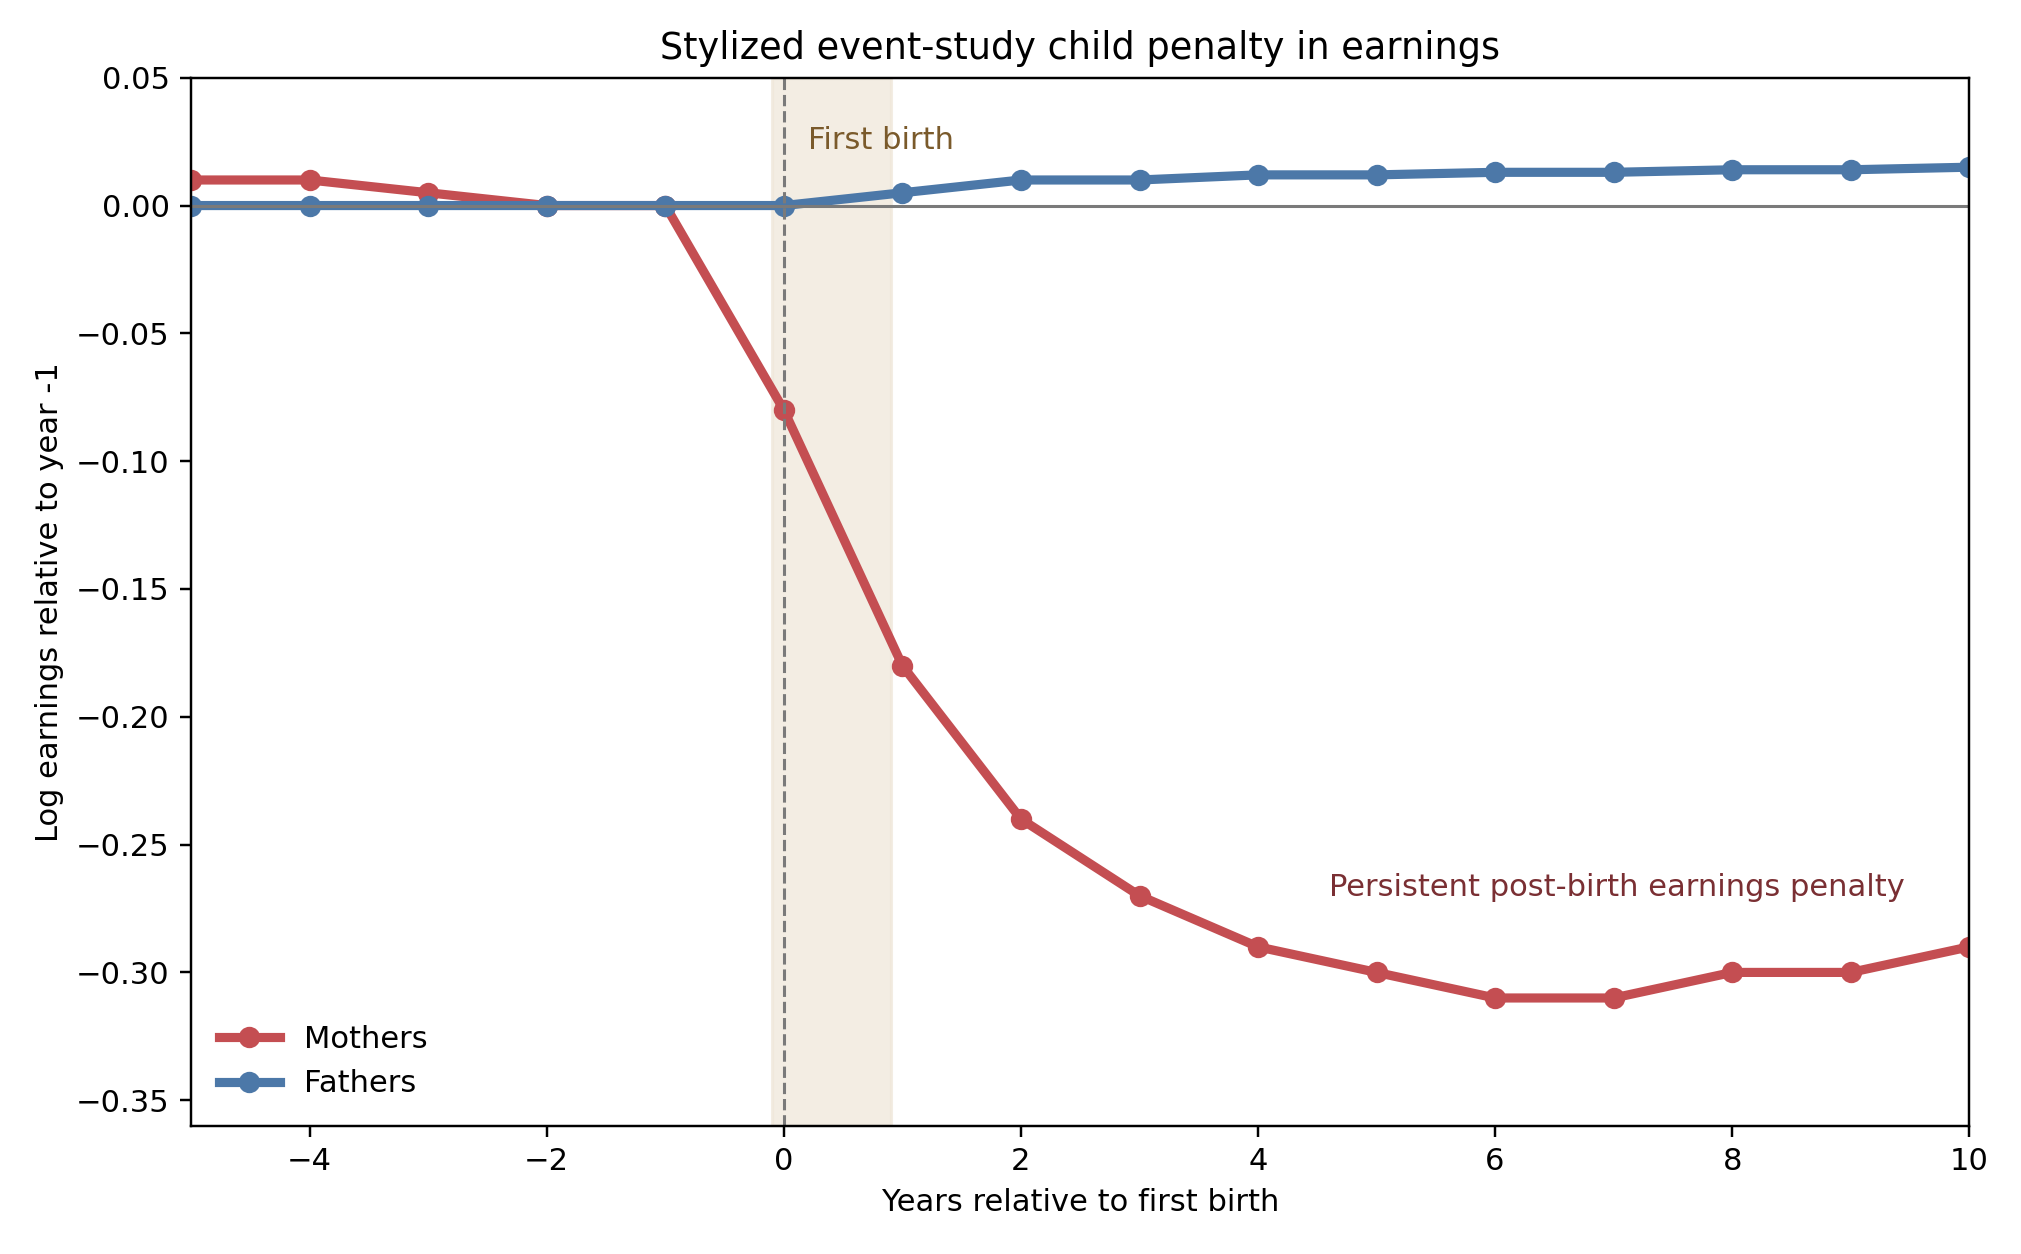
\includegraphics[height=0.74\textheight,keepaspectratio]{06-child-penalty-event-study.png}
\end{center}
\end{frame}

\begin{frame}{Policy-margin map}
\scriptsize
\begin{tabular}{p{0.21\linewidth} p{0.18\linewidth} p{0.17\linewidth} p{0.21\linewidth} p{0.17\linewidth}}
\toprule
Policy or shock & Primary margin & Secondary margin & Outcomes & Week 6 use \\
\midrule
Childbirth shock & Participation and hours & Wage growth, occupation, firm choice & Employment, earnings, wages & Fertility IV and child penalties \\
Childcare access & Participation & Hours and re-entry & Employment, hours, childcare use & Childcare designs \\
Public school entry & Participation & Timing of work & Maternal labor supply & Gelbach-style threshold \\
Parental leave & Short-run attachment & Long-run earnings path & Leave, retention, earnings & Family-policy extensions \\
Income to one spouse & Intra-household allocation & Labor supply and spending & Hours, expenditures & Pooling versus bargaining tests \\
Cheaper services & Intensive margin & Leisure and housework & Hours and housework & Outsourcing channel \\
\bottomrule
\end{tabular}
\end{frame}

\begin{frame}{Bridge to Week 7 and Week 8}
\begin{itemize}
    \item Week 7: flexibility, schedule control, and remote work become household inputs once care constraints bind.
    \item Week 8: earnings inequality partly reflects fertility timing, care institutions, and household responses rather than only skill prices.
    \item Household structure is therefore central to both compensating differentials and modern inequality accounting.
\end{itemize}
\end{frame}

\begin{frame}{Takeaways}
\begin{itemize}
    \item Family labor supply is jointly produced through wages, care needs, and household technology.
    \item Unitary and collective models imply different tests and different policy incidence.
    \item Fertility IV and child-event-study designs recover different but complementary objects.
    \item Week 6 is the bridge from worker-side labor supply to amenities and inequality.
\end{itemize}
\end{frame}

\appendix

\begin{frame}{Appendix: optional extension block}
\begin{itemize}
    \item Relative-income constraints and household norms in the spirit of Bertrand, Kamenica, and Pan.
    \item Long-run family-policy experimentation in the spirit of Kleven et al. (2024).
    \item Optional lab reflection: which policies change the home-production technology and which change bargaining weights?
\end{itemize}
\end{frame}

\end{document}
